% !Mode\dots ``TeX:UTF-8''
% !TEX root = ../root.tex
\section{Determining the online observability of \BCNs}
\label{sec:deter}
After defining the online observability and comparing it with the existing four observability, we propose two algorithms to determine the online observability of \BCNs. The first one is the supertree-based algorithm, and the second one is the algorithm based on directed graph. Based on the definition of online observability, we propose the supertree to describe the process of determining the initial state of a \BCN. And then, we propose the algorithm to determine the online observability of \BCNs\ based on the supertree. But the supertree-based algorithm can not help us find all paths to determine the initial state of a \BCN. In order to improve the shortcomings of the supertree-based algorithm, we propose the algorithm based on directed graph. The algorithm based on directed graph may take longer time for us to determine its online observability. But if we want do some optimizationin in the process of determining the initial state of a \BCN, this algorithm would be better. What is more, we also analyze the complexity of the algorithm based on directed graph in this section. Finally, we represent how to determine the initial state of a \BCN\ by the directed graph.
%The construction processes of supertree and directed graph simulate derivation process of the initial state mentioned before. We check the super tree based on the definition of online observability of \BCNs\ depth first or breadth first. When we find enough leaf nodes, we can make sure the \BCN\ is online observable. But when we use the super tree to find all paths to determine the initial state of a \BCN, we need to check the existence of loops when we build the super tree. And many nodes in the tree are repeated, these nodes will take a lot of time overhead and space overhead for us to build and check the super tree for \BCNs. Therefore, we proposed the second way to determine the online observability of \BCNs\ by using directed graph. By this way we can avoid checking the existence of loop and avoid checking repeated nodes. There are also other advantages which help us select the input better in the process of determining the initial state of a \BCN\ by the second way. All of these advantages will reduce time and space overhead to determine the initial state of a \BCN. In conclusion if a \BCN\ seems to be online observable we would check it earlier by using supertree. But if a  \BCN\ does not seem to be online observable we prefer to check it earlier by using directed graph. If we just want to find a path to determine the initial state of a \BCN\ we would check it by using supertree. But if we want find all paths to determine the initial state of a \BCN\ and make some optimizations in the process of determine the initial state we prefer to check tthe \BCN\ by using directed graph.

\subsection{Supertree-based algorithm} %As we mentioned before, we can use the derivation function to determine the initial state of \BCNs. 
According to the definition of online observability, we alternately observe the output and then derive and decide the input in the process of determining the initial state of a \BCN. When the  cardinal number of the set of possible states comes into be $1$, we can determine the current state of this \BCN\ and then its initial state. We define the supertree for \BCNs\ to describe this process, and then propose the supertree-based algorithm to determine the online observability for \BCNs. For convenience, we use the set of state $S_i$ inside a node to represent this node, and the input $i_p$ or output $o_j$ in an edge to represent the edge.
\begin{definition}[Supertree]
For a \BCN, every node $S_i$ in the supertree is $K$-step deterministic. The root node of its supertree is $\Delta_N$, while the leaf nodes of the supertree are the nodes with cardinal number $1$ ($|S_i|=1$). In addition to the leaf nodes, if a node $S_i$ in the $2k + 1$ ($k\in \mathbb{N}$) layer of the supertree and 
\[|\Ded\left(S_i,\varepsilon, o_j\right)|>0,\]
 then $\Ded\left(S_i,\varepsilon, o_j\right)$ is one of its son nodes, and $o_j$ is the edge from $S_i$ to $\Ded\left(S_i,\varepsilon, o_j\right)$ for each $o_j \in \Delta_Q$. If a node $S_i$ in the $2k+2$ layer of the supertree and  
\[|\Ded\left(S_i,i_p,\varepsilon\right)|=|S_i|,\] 
then $\Ded\left(S_i,i_p,\varepsilon\right)$ is the son node of $S_i$ and $i_p$ is the edge from $S_i$ to $\Ded\left(S_i,i_p,\varepsilon\right)$ for each $i_p \in \Delta_M$. 
\label{def:super-tree}
\end{definition}

  \begin{figure}[thpb]
      \centering
      \framebox{\parbox{3in}{
		\centerline{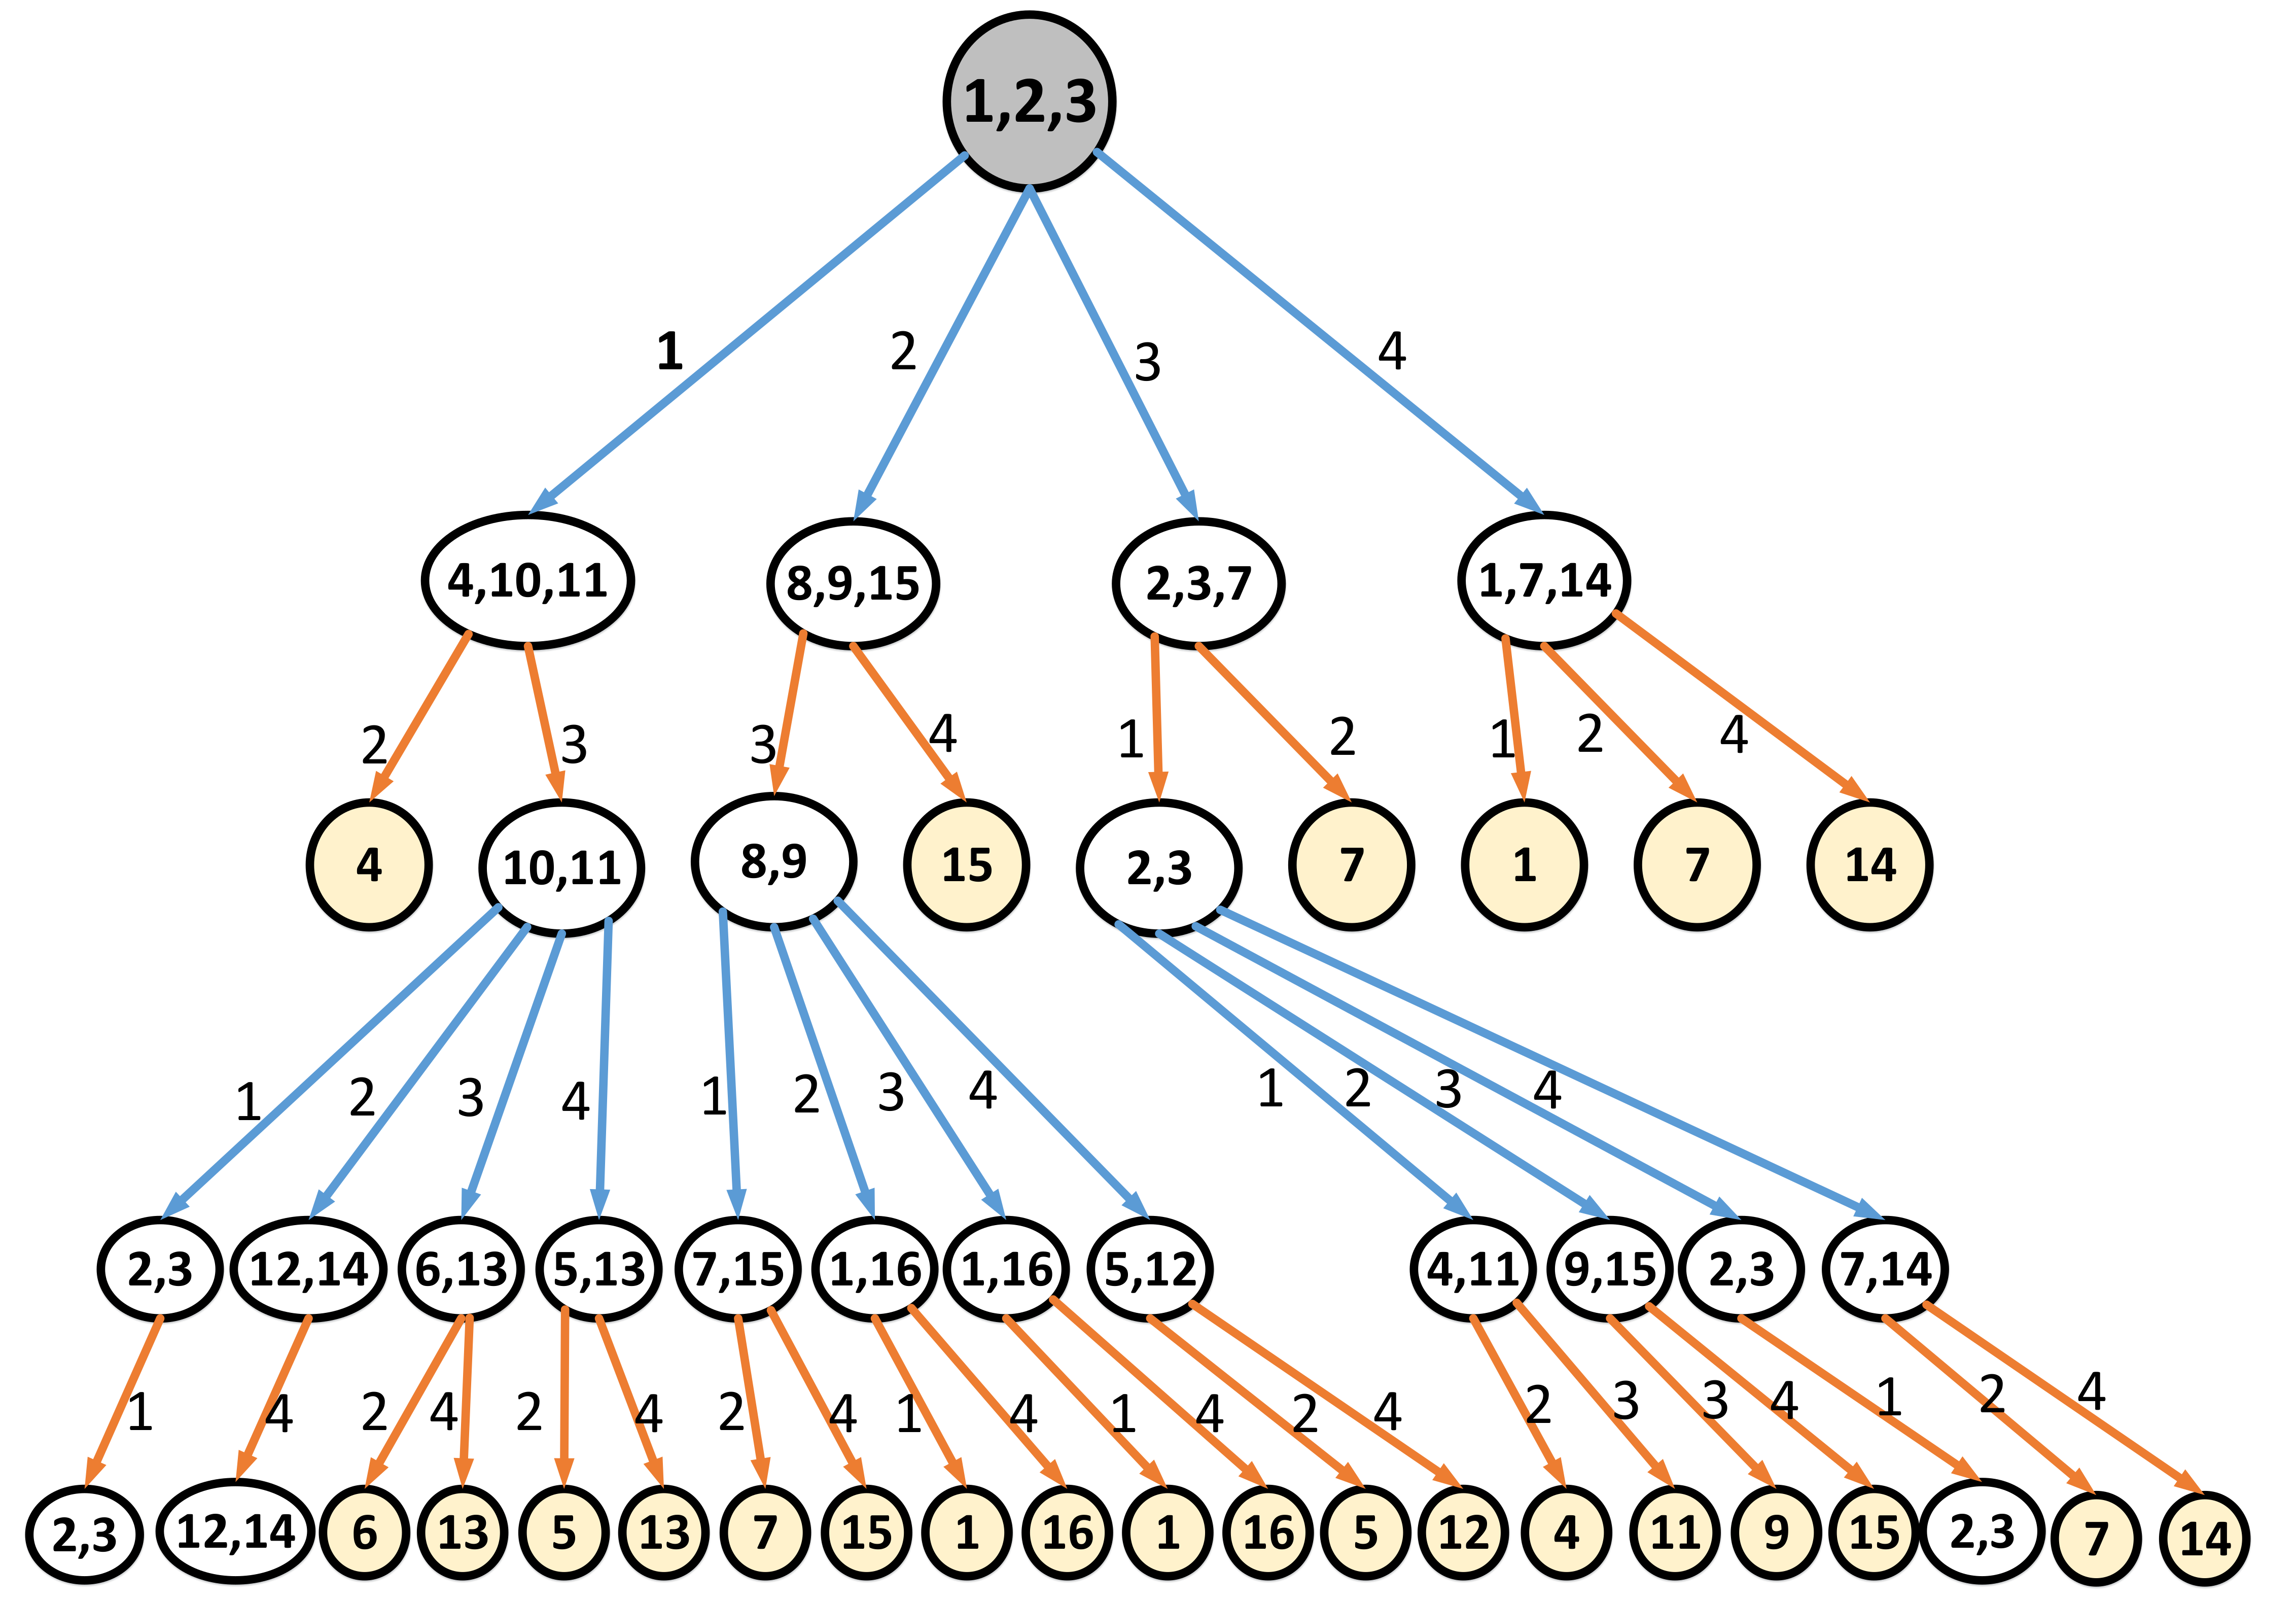
\includegraphics[scale=0.067]{figures/Fig3.png}}
	}}
      
      \caption{Branch of the super tree which represents $\{\delta_{16}^1,\delta_{16}^2,\delta_{16}^3\}$. The blue edges and orange edges show the observing output processes and deciding input processes, respectively. The yellow nodes are leaf nodes.}
      \label{fig:3}
   \end{figure}

In the {\em Definition \ref{def:super-tree}}. For a \BCN, we can only infer that the possible states set is $\Delta_N$ at the beginning, thus the root node of the super tree is $\Delta_N$. And then,  we can determine the state of the \BCN\ when the cardinal number of the possible states set turns into $1$. Therefore, the leaf nodes of the supertree are the nodes with cadinal number $1$. In the process of determining the initial state of a \BCN, we observe the output of the \BCN\ to derive the set of possible states at first. After that, we derive and decide the input and then derive the new possible states set of the \BCN. We alternately observe the output and then derive and decide the input untill we can determine the state of {\em BCN}. Therefore we use $\Ded\left(S_i,\varepsilon, o_j\right)$ to find child nodes for every $S_i$ in $2k+1$ layer, and using $\Ded\left(S_i,i_p,\varepsilon\right)$ to find child nodes for every $S_i$ in $2k+2$ layer. The formula 
\[|\Ded\left(S_i,\varepsilon, o_j\right)|>0\]
 ensures the node $\Ded\left(S_i,\varepsilon, o_j\right)$ is not empty. The formula 
 \[|\Ded\left(S_i,i_p,\varepsilon\right)|=|S_i|\] 
 guarantee we can determine the state of \BCN\ in the end ({\em Section \ref{sec:online}} {\em Equation \ref{equ:12}}). Therefore, the paths to determine the initial state of a \BCN\ are described in the supertree, and then we can use it to determine the online observability for a \BCN.

Based on the definition of the supertree, we propose the supertree-based algorithm ({\em Algorithm.\ref{alg:3}}) to determine the online observability for \BCNs. 
%If we want to find all of the ways to determine the initial state of a \BCN, we have to build all leaf nodes for the super tree of this \BCN. This process takes many additional time and space overhead. Especially when there are loops in the tree such as the $\{\delta_{16}^2,\delta_{16}^3\}$ in fourth layer and the $\{\delta_{16}^2,\delta_{16}^3\}$ in fifth layer which will form a loop. In this case we can never build the complete tree, thus we need to check the existence of loops and omit them. There are also some nodes take the same set of state, that they will take some additional overhead as well. For instance there are two nodes take the same states set $\{\delta_{16}^1,\delta_{16}^{16}\}$ in the fifth layer. However, using super tree would be a lot easier than using directed graph if we only need to find a way to determine the initial state. For instance, when we find the leaf nodes $\delta_{16}^1$, $\delta_{16}^7$ and  $\delta_{16}^{14}$ in third layer by breadth-first algorithm, we can make sure that the states set $\{\delta_{16}^1,\delta_{16}^2,\delta_{16}^3\}$ is 1 step deterministic. Therefore, we could use this conclusion to determine the initial state of this \BCN. 
\begin{algorithm}[h]
\caption{Supertree-based algorithm}
\begin{algorithmic}[1]
\REQUIRE 
The algebraic form of \BCN
\ENSURE  
The super tree of \BCN
%\STATE  $k=1$ \
\STATE  $Ob=$ false %(The online observability of \BCN)\
%\STATE  $N_i$ (Node)\
%\STATE  $i_p$ (Input)\
\STATE  $NodesArray$ =$\Delta_N$\
%\STATE  $Sis$ (The suitable inputs set of $N_i$)\
%\STATE {\sf buildnode}(k)
%\STATE $k= k+1$
\WHILE {$Ob==$ false}
\STATE Build child nodes for $NodesArray$ by $\Ded\left(S_i,\varepsilon, o_j\right)$
\STATE $NodesArray=$ Child nodes of $NodeArray$ except leaf nodes
\STATE Check this \BCN\ by the super tree
\IF{\BCN\ is online observable}
\STATE $Ob=$ true
\ELSE
\STATE Build child nodes for $NodesArray$ by $\Ded\left(S_i,i_p,\varepsilon\right)$
\STATE $NodesArray=$ Child nodes of $NodeArray$
\ENDIF
\ENDWHILE
\STATE Delete uncertain branches
\STATE  $NodesArray$ =$\Delta_N$\
%\STATE return $Ob$
\STATE return $NodesArray$
\end{algorithmic}
 \label{alg:3}
\end{algorithm}

In the supertree-based algorithm we build trees by breadth first. We check the online observability of the \BCN\ by the supertree after $2k+2$ layer of the supertree was built for every $k\in  \mathbb{N}$. If the \BCN\ is online observable, then we stop building the supertree and delete the uncertain branches. Finally, we return the $NodesArray$ which is the root node of the supertree, and then we can determine the initial state of the \BCN\ by the supertree.

In order to better illustrate how to use the super tree to determine the online observability, we give the following example.
  
\begin{example}
In the \BCN\ mentioned in {\em Example \ref{exa:2}}. From the definition of online observability we need to determine whether the $\Ded\left(\Delta_N,\varepsilon,o_j\right)$ is $K$-step deterministic for every  $o_j \in \Delta_Q$ such that $|\Ded\left(\Delta_N,\varepsilon, o_j\right)|> 0$. Therefore, we build child nodes for $\Delta_N$ by the $\Ded\left(S_i,\varepsilon, o_j\right)$. For instance, \[\Ded\left(\Delta_N,\varepsilon,\delta_{4}^1\right)=\{\delta_{16}^1,\delta_{16}^2,\delta_{16}^3\}\] and we can not determine whether $\{\delta_{16}^1,\delta_{16}^2,\delta_{16}^3\}$ is $K$-step deterministic or not, and then we can not determine the online observability of this \BCN\ by the supertree now. Therefore we build child nodes for it, and then build child nodes for its child nodes as shown in the Fig.\ref{fig:3}. Then we check the second and third layer of this branch, we have the nodes $\{\delta_{16}^1\}$, $\{\delta_{16}^7\}$ and $\{\delta_{16}^{14}\}$ are $K$-step deterministic, and then we have the node $\{\delta_{16}^1,\delta_{16}^2,\delta_{16}^3\}$ is $K$-step deterministic. We use the same method to check other nodes, and then determine the online observability for the \BCN. Finally, we delete uncertain branches except the branches which can help us to determine online observability, such as the first branch ($\{\delta_{16}^{4},\delta_{16}^{10},\delta_{16}^{11}\}$). And then, the supertree can help us to determine the initial state of the \BCN.%We can also determine the initial state of this \BCN\ by this branch.The nodes represent the sets of possible states, the blue edges represent the processes of observing output, and the orange edges represent the processes of deriving and deciding input. Only the yellow nodes are the leaf nodes, thus this branch is not completed. %When we check the second and third layer of this branch, we have the nodes $\{\delta_{16}^1\}$, $\{\delta_{16}^7\}$ and $\{\delta_{16}^{14}\}$ are $K$-step deterministic, and then we have the node $\{\delta_{16}^1,\delta_{16}^2,\delta_{16}^3\}$ is $K$-step deterministic. We can also determine the initial state of this \BCN\ by this branch.

\end{example}   

However, if we want use the supertree-based algorithm to find all paths to determine the initial state of a \BCN. In this case, we need to check the nodes that appear multiple times in the supertree, and this nodes would take many additional time and space overhead. For instance, in the Fig.\ref{fig:3} there are two nodes take $\{\delta_{16}^1,\delta_{16}^{16}\}$ in the fourth layer. Moreover, the same nodes in a path will form a loop, the loops in the supertree will prevent us from building a complete tree. For example, there are the $\{\delta_{16}^2,\delta_{16}^3\}$ in fourth layer and the $\{\delta_{16}^2,\delta_{16}^3\}$ in fifth layer, and they would form a loop. With the shortcomings of the supertree, we propose the algorithm based on directed graph to help us find all paths to determine the initial state of a \BCN.
\subsection{Algorithm based on directed graph}
In order to improve the shortcomings of the supertree-based algorithm, we proposed the algorithm based on directed graph. The biggest difference of these two algorithms is the way how the  supertree and derected graph constructed. That supertree is built from the root node ($\Delta_N$) to leaf nodes (contain 1 state), while the derected graph is built from smallest nodes (contain 1 state) to largest node (contain largest number of states). In addition, there is not any repeated node in the derected graph because every node appears only once in the directed graph. What is more, even there are some loops in the derected graph, the loops would not prevent us from building the directed graph completely.

Therefore, we have the definition of directed graph for \BCNs.
\begin{definition}[Directed Graph]
Firstly, every node $S_i$ in the directed graph is $K$-step deterministic, and there are no duplicate nodes in the graph. 

Secondly, for every node $S_i$  and $|S_i|>1$, we have that for every distinct two $s_a, s_b \in S_i$, $Hs_a=Hs_b$. 

Finally, fot the edges of the directed graph. 
\begin{itemize}
 \item If $|S_i|=1$, then there are not edge from it to other nodes.
 \item  If $|S_i|>1$, and there are exist one edge $i_p$ from it to one nodes, then there exist $z\ge 1$ such that there are $z$ edges contain $i_p$ from it to nodes $S_1,\ldots,S_z$ that \[|S_i|= |S_1|+,\ldots,|S_z|\] and \[\Ded\left(S_i,i_p,\varepsilon\right)=S_1\vee,\ldots,\vee S_z.\]
 \end{itemize}

\end{definition}

From the {\em Lemma \ref{lemm:5}} in the {\em Section \ref{sec:online}}, we have that if the set of states $S_i$ is not $K$-step deterministic and $S_i\subset S_j$, then $S_j$ is not $K$-step deterministic. Therefore, we check whether the nodes with fewer states are $K$-step deterministic at first, and then we check whether the nodes with more states are $K$-step deterministic in the process of building the directed graph for a \BCN. Once we can find a node $S_i$ is not $K$-step deterministic, then we make sure that there exists $o_j \in \Delta_Q$ such that $|\Ded\left(\Delta_N,\varepsilon, o_j\right)|> 0$ and $S_i\subset \Ded\left(\Delta_N,\varepsilon, o_j\right)$, then $\Ded\left(\Delta_N,\varepsilon,o_j\right)$ is not $K$-step deterministic, and then this \BCN\ is not online observable. %Moreover, we can use the nodes with fewer states that are $k$-step deterministic to help us check the nodes with more states. For instance, if the node $S$ has two edges from it to two nodes $S_1$ and $S_2$, and we have $S_1$ and $S_2$ are $k$-step deterministic. In this case, we can make sure that the node $S$ is $k$-step deterministic.

With the definition of directed graph and the way to construct the derected graph. We propose the algorithm based on directed graph prsented in the {\em Algorithm.\ref{alg:1}}. And the {\em Algorithm.\ref{alg:2}} present the algorithm to build nodes which is used in the {\em Algorithm.\ref{alg:1}}.

\begin{algorithm}[h]
\caption{Algorithm based on directed graph}
\begin{algorithmic}[1]
\REQUIRE 
The algebraic forms of \BCN
\ENSURE  
The directed graph of \BCN
\STATE  $k=1$ %(The number of states in the nodes)\
\STATE  $Ob=$ true %(The online observability of \BCN)\
%\STATE  $N_i$ %(Node)\
%\STATE  $i_p$ %(Input)\
%\STATE  $NodesArray$% (Nodes array)\
%\STATE  $Sis$ %(The suitable inputs set of $N_i$)\
\STATE {\sf buildnode}(k)
\STATE $k= k+1$
\STATE $NodesArray=${\sf buildnode}(k)
\WHILE {$NodesArray!=$Null}

\FOR{each $S_i\in NodesArray$}
\IF{$k==2$}
\STATE $Sis$ = $\Delta_M$ 
\ELSE

\STATE Find $Sis$ by other nodes

\ENDIF
\FOR{each $i_p \in Sis$}
\STATE Check $S_i$ by $i_p$
\STATE Build edges for $S_i$ 
\ENDFOR
\IF {$S_i$ has not any edge.}
\STATE  $Ob=$ false 
\STATE return Null
\ENDIF
\ENDFOR
\STATE $k= k+1$
\STATE $NodesArray=${\sf buildnode}(k)
\ENDWHILE
%\STATE $Ob=1$ 
\STATE $NodesArray=${\sf buildnode}(k-1)
\STATE return $NodesArray$
\end{algorithmic}
 \label{alg:1}
\end{algorithm}
 %The algorithm to build nodes used in the Algorithm.\ref{alg:1} is shown in the Algorithm.\ref{alg:2}.
\begin{algorithm}[h!]
\caption{{\sf buildnode}(int k)}
\begin{algorithmic}[1]
\REQUIRE 
The number of states $k$
\ENSURE  
The nodes with $k$ states which with the same corresponding outputs %, and the outputs of $p$ states inside one node are the same.
%\STATE {\sf buildnode}(int p)
%\STATE  \{ 
%\dfSTATE $p=p+1$\
\STATE  Build all nodes with $p$ states %(whose outputs are the same)\

\IF{Failed to build} 
\STATE  return Null
\ELSE 
\STATE  Classify these nodes
\STATE Sort the states in these nodes
\STATE Sort these nodes%(For example, the nodes $\{\delta_{16}^1,\delta_{16}^2\}$, $\{\delta_{16}^1,\delta_{16}^3\}$ and $\{\delta_{16}^2,\delta_{16}^3\}$ shown in {\em Fig.\ref{fig:4}}. )
\STATE return nodes
\ENDIF 
%\STATE \}
\end{algorithmic}
 \label{alg:2}
\end{algorithm}
%%\newpage

There are some details in {\em Algorithm.\ref{alg:1}} and {\em Algorithm.\ref{alg:2}} are as follows:
\begin{itemize}
\item Build all nodes with $k$ states: Firstly, we classify all states by their corresponding outputs ($\Ded\left(\Delta_N,\varepsilon,o_j\right)$), then we have all of the states sets. The states set contains all states that with the same corresponding outputs. Secondly, we compare $k$ with the cardinal number $|\Ded\left(\Delta_N,\varepsilon,o_j\right)|$ of each states set we built before. If $k$ greater than $|\Ded\left(\Delta_N,\varepsilon,o_j\right)|$, then we could not get $k$ states from this states set. Else we can get $C_{|\Ded\left(\Delta_N,\varepsilon,o_j\right)|}^k$ sets with $k$ states from this states set. Finally, we use all of the sets of states found in second step to build nodes we need. 
 \item Sort the states in these nodes and sort these nodes: For example, the nodes $\{\delta_{16}^1,\delta_{16}^2\}$, $\{\delta_{16}^1,\delta_{16}^3\}$ and $\{\delta_{16}^2,\delta_{16}^3\}$ shown in Fig.\ref{fig:4}. We sort the states inside the nodes at first, and then sort the nodes by the states of them.
  \item Find $Sis$ by other nodes: From the {\em Lemma \ref{lemm:4}} and {\em Lemma \ref{lemm:3}} in the {\em Section \ref{sec:online}}, we have if $S_i\subset S_j$ then for any input $i$ wich can not make $S_i$ $K$-step deterministic, it can not make $S_j$ $K$-step deterministic either. Therefor, for the node $S_i$ with $k$ sorted states inside it, we can use the node with the first $k-1$ states of $S_i$ and the node with the last $k-1$ states of $S_i$ to find the suitable inputs set $Sis$ for $S_i$. For example, we can search correct inputs sets which make $\{\delta_{16}^4,\delta_{16}^5,\delta_{16}^6\}$ and $\{\delta_{16}^5,\delta_{16}^6,\delta_{16}^7\}$ $K$-step deterministic at first. After that, take the intersection of these sets to be the suitable inputs set of $\{\delta_{16}^4,\delta_{16}^5,\delta_{16}^6,\delta_{16}^7\}$. 
  \item Check $S_i$ by $i_p$: According to the order determined in previous steps, we check every node in order. If for one input $i_p\in Sis$ implies $|\Ded\left(S_i,i_p,\varepsilon\right)|<|S_i|$, we can make sure the $i_p$ is a wrong input. Else if for each $O_j \in \Delta_Q$, $|\Ded\left(S_i,i_p,o_j\right)|>0$ and $\Ded\left(S_i,i_p,o_j\right)$ is $K$-step deterministic then $I_j$ is a correct input. Therefore, we can connect the node $S_i$ to each node $\Ded\left(S_i,i_p,o_j\right)$ with directed edge. Else if there exist $o_j \in \Delta_Q$ and we can not make sure whether $\Ded\left(S_i,i_p,o_j\right)$ is $K$-step deterministic, then we check it in the next round. 
\end{itemize} 

\begin{figure}[thpb]
      \centering
      \framebox{\parbox{3in}{
		\centerline{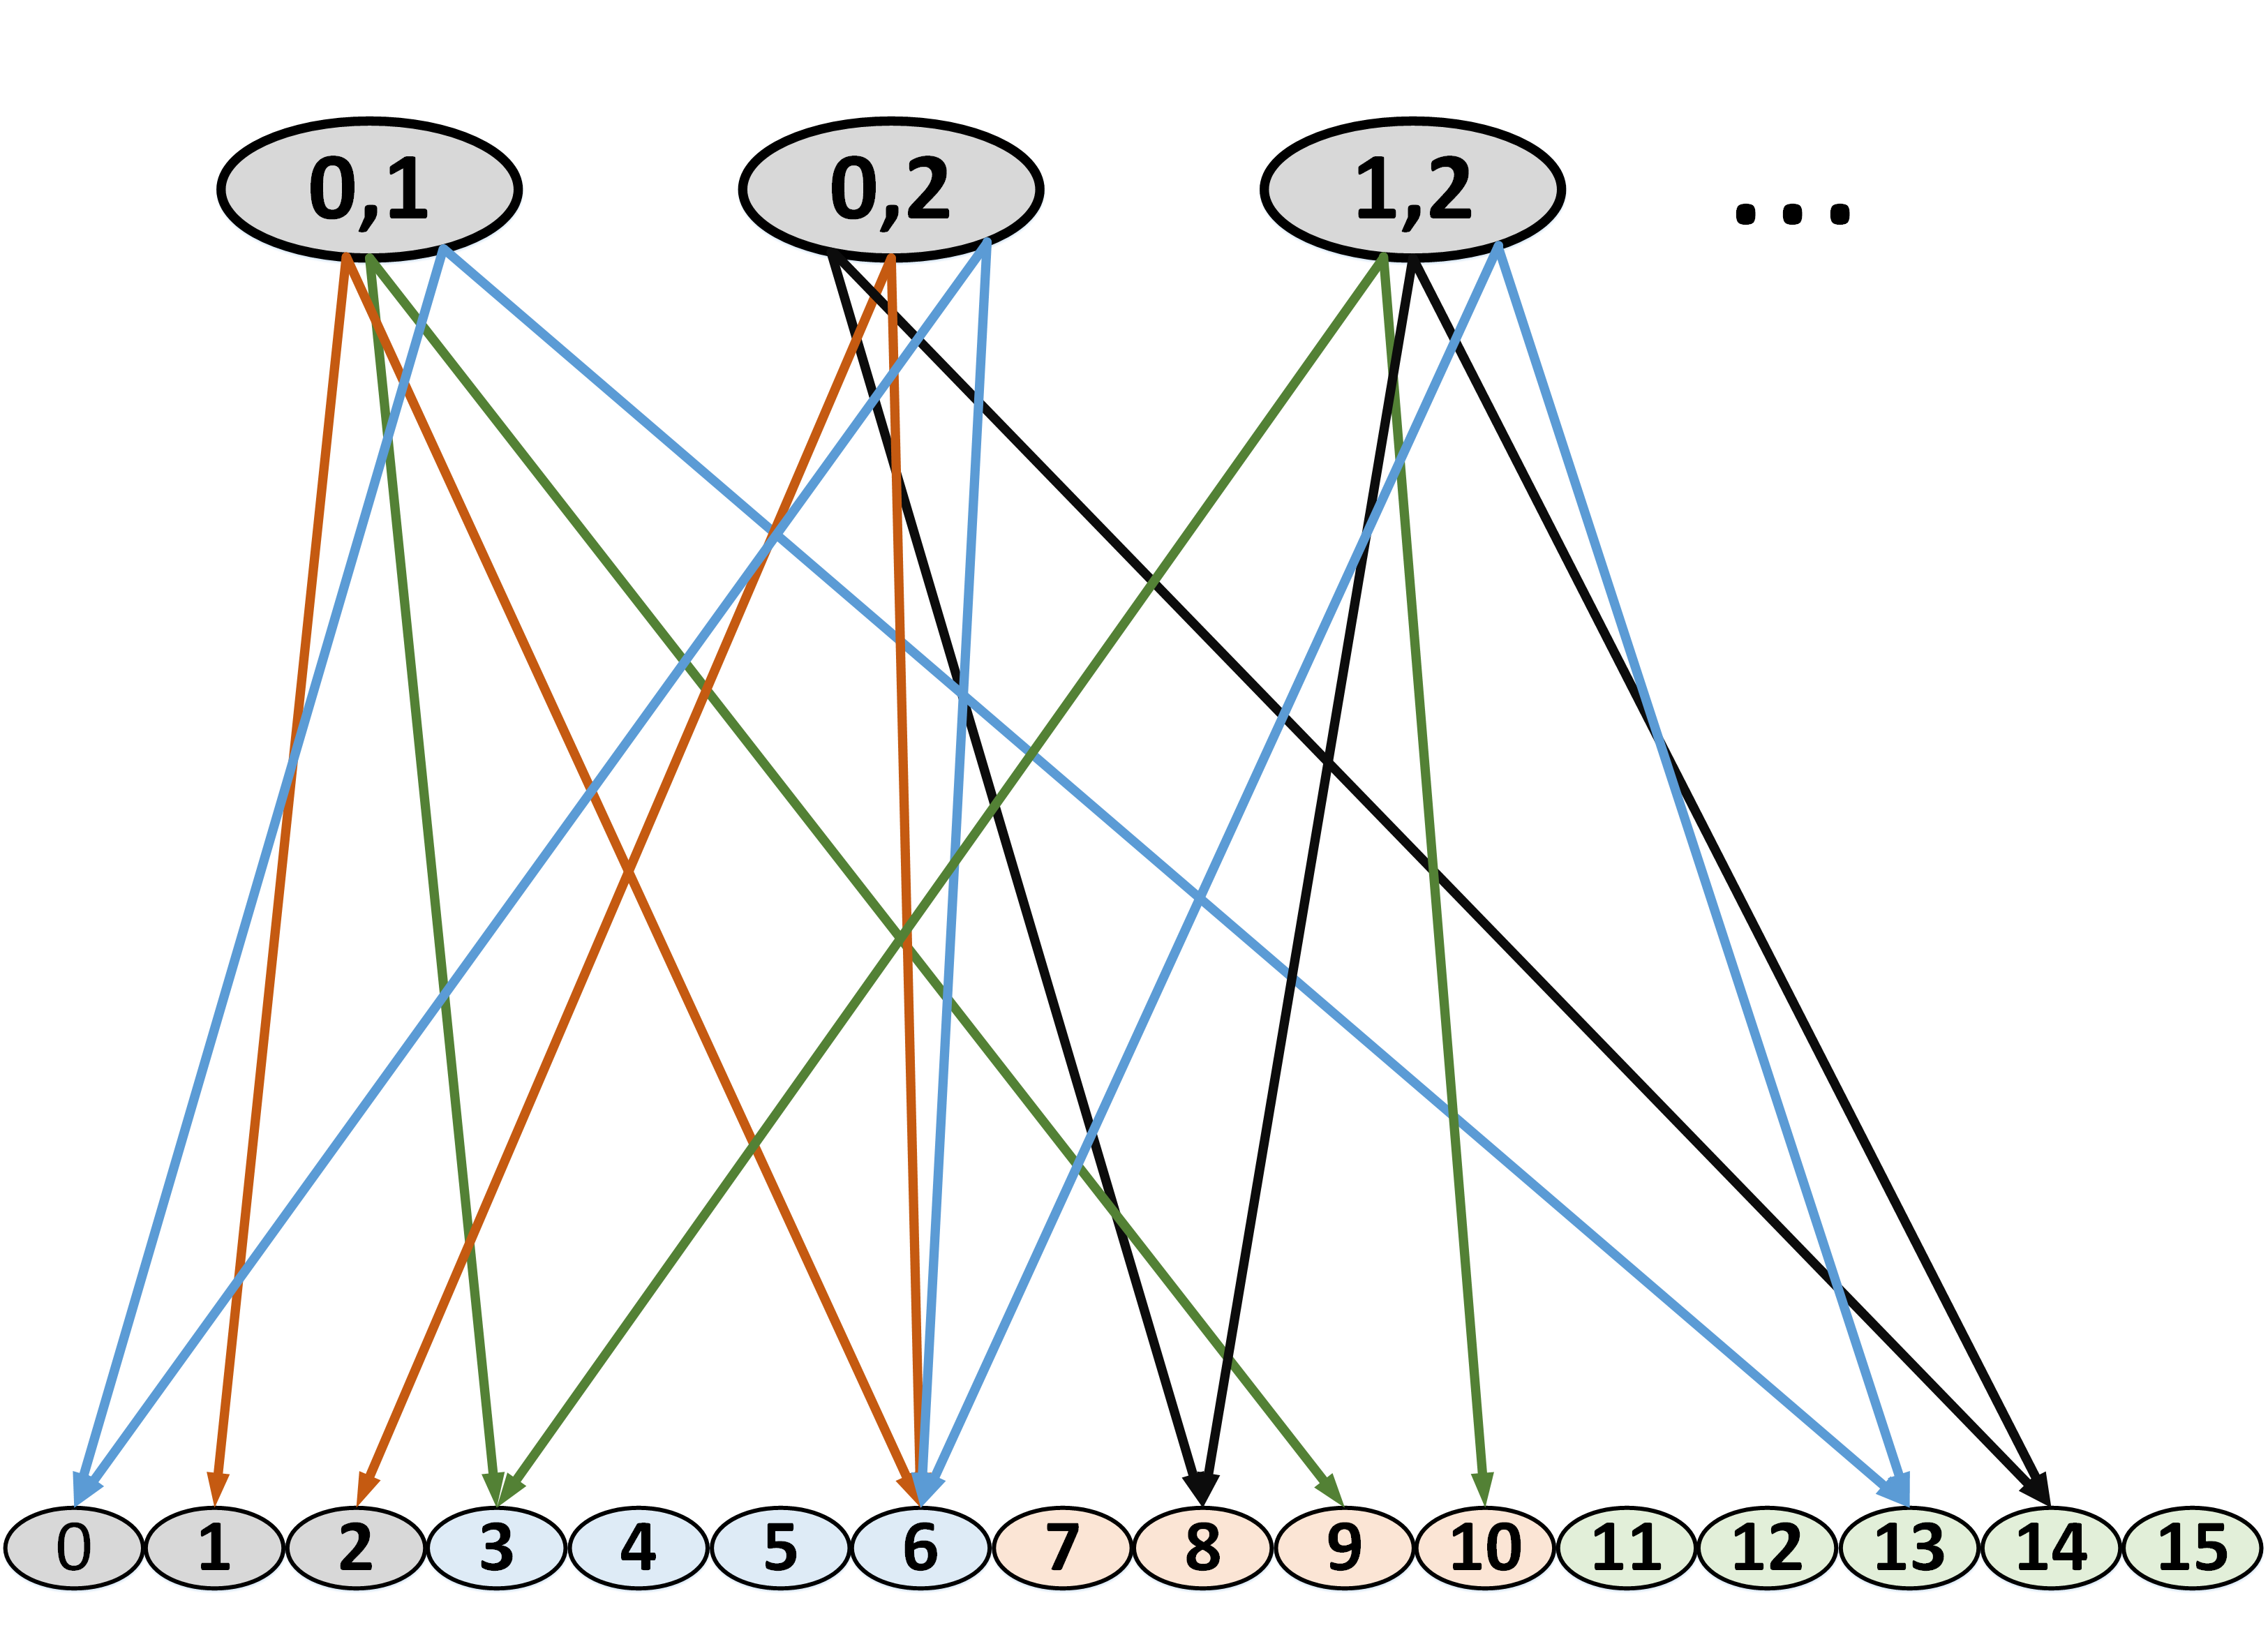
\includegraphics[scale=0.090]{figures/Fig4.png}}
	}}
      
      \caption{Part of the directed graph which represents $\{\delta_{16}^1,\delta_{16}^2\}$, $\{\delta_{16}^1,\delta_{16}^3\}$ and $\{\delta_{16}^2,\delta_{16}^3\}$. The green, black, orange, blue edges show the inputs $\delta_4^1$, $\delta_4^2$, $\delta_4^3$ and $\delta_4^4$ respectively.}
      \label{fig:4}
   \end{figure}

What is more, based on the definitions of existing four types of observability, we can also use the directed graph to determine the existing second and fourth type of observability for \BCNs. 
\begin{itemize}
 \item Checking the existing second observability: When we try to build bottom layer and penultimate layer of the directed graph, and there are exist some nodes in penultimate layer has no edges from it to other nodes. 
 Therefore, there are distinct states $s_0$, ${s'}_0 \in \Delta_N$, and there does not exist any input sequence $I\in(\Delta_M)^p$ for any $p\in \mathbb{Z}_+$, such that $Hs_0=H{s'}_0$ implies $(HL)^p_{s_0}(I)\neq (HL)^p_{{s'}_0}(I)$.
 And then, this \BCN\ does not satisfy existing second observability.
 \item  Checking the existing fourth observability: When we try to build edges for every layer, and if there exist one node whose right inputs set is not $\Delta_M$, 
 then there exists an input sequence $I\in(\Delta_M)^{\infty}$ does not satisfy that for any distinct states $s_0$, ${s'}_0 \in \Delta_N$, $Hs_0=H{s'}_0$ implies $(HL)^{\infty}_{s_0}(I)\neq (HL)^{\infty}_{{s'}_0}(I)$. And then this \BCN\ does not satisfy existing fourth observability.
 \end{itemize}



\subsection{Complexity analysis}
As the algorithm by the directed graph is better than by supertree when we want to find all paths to determine the initial state of \BCNs. We analyze the complexity of this algorithm briefly in this paper. 
%We classify the states with their corresponding output . After that form the set of states set $\{\Ded\left(\Delta_N,\varepsilon,\delta_M^1\right), \Ded\left(\Delta_N,\varepsilon,\delta_M^2\right),\ldots,\Ded\left(\Delta_N,\varepsilon,\delta_M^M\right)\}$, then every element in a states set has the same corresponding output. For each \[S_i\in\{\Ded\left(\Delta_N,\varepsilon,\delta_M^1\right), \Ded\left(\Delta_N,\varepsilon,\delta_M^2\right),\ldots,\Ded\left(\Delta_N,\varepsilon,\delta_M^M\right)\}\] we have $Hs_k=\delta_{M}^i$ for every $s_k\in S_i$.
\begin{itemize}
\item Firstly, we need to calculate the number of layers in the directed graph i.e. the upper bound of the number ($k$) of the states of the nodes in the directed graph. We have that 
\begin{equation}
\begin{split}
k_{upb}= \max(|\Ded\left(\Delta_N,\varepsilon,\delta_M^1\right)|,\ldots,|\Ded\left(\Delta_N,\varepsilon,\delta_M^M\right)|).
\end{split}
\end{equation}
%The upper bound of the number of the states of the nodes in the directed graph $k_{upb}$ is the maximum value of $|\Ded\left(\Delta_N,\varepsilon,\delta_M^1\right)|,\ldots,|\Ded\left(\Delta_N,\varepsilon,\delta_M^M\right)|$, 
Because the states of the same nodes in the directed graph should have the same corresponding output. Therefore, the $k_{upb}$ indicates the number of layers in the directed graph, and it depends on the relationship between states and outputs of the \BCNs.

\item Secondly, we need to calculate the number of nodes which with $k$ states, we have that
\begin{equation}
\begin{split}
Non(k)= C_{|S_i|}^k+\ldots +C_{|S_p|}^k,
\end{split}
\end{equation}
where \[S_i\ldots,S_p\in\{\Ded\left(\Delta_N,\varepsilon,\delta_M^1\right),\ldots,\Ded\left(\Delta_N,\varepsilon,\delta_M^M\right)\}\] and $|S_i|,\ldots,|S_p|\ge k$. The $Non(k)$ indicates the number of nodes which built by the {\sf buildnode}(k) function, and it also depends on the relationship between states and outputs of the \BCNs.

\item Thirdly, we need to calculate the cardinal number of suitable inputs set of each node $|Sis(S_i)|$. If $|S_i|=2$ then $Sis(S_i)=\Delta_M$. If $|S_i|>2$ then $Sis(S_i)$ is derived by other nodes, therefore it depends on the updating rules of the \BCNs.

\item Finally, we need to calculate the time used to check whether a input which in the suitable inputs set of a node is a right input for this node $T(S_i, i_p)$, and it depends on the updating rules of the \BCNs\ as well.
 \end{itemize}

After completing the previous analysis, we calculate the complexity by layer by layer, then we have the time we need to determine the online observability.  
\[T=\sum_{k=1}^{k_{upg}}\sum_{i=1}^{Non(k)}\sum_{p=1}^{Sis(S_i)}T(S_i, i_p)\]
%The cardinal number of suitable inputs set of a node depends on the cardinal number of this node and the other three nodes used to find the suitable inputs set for it. And the time used to check whether an input is a right input for a node also depends on the updating rules of {\em BCNs}.

%What is more, instead of taking $\Delta_M$ as the suitable inputs set for every node in thedirected graph, we use the other three nodes like $\{\delta_{16}^4,\delta_{16}^5,\delta_{16}^6\}$, $\{\delta_{16}^5,\delta_{16}^6,\delta_{16}^7\}$ and $\{\delta_{16}^4,\delta_{16}^7\}$ that are $k$-step deterministic to find the suitable inputs set for a node $\{\delta_{16}^4,\delta_{16}^5,\delta_{16}^6,\delta_{16}^7\}$ which with more than $2$ states. By this way we can  reduce the cardinal number of the suitable inputs set for every nodes with more than 2 states, and then reduce the time cost. 

%The reason why we can use this method is that only the input which make the subset of $\{\delta_{16}^4,\delta_{16}^5,\delta_{16}^6,\delta_{16}^7\}$ $k$-step deterministic will make the $\{\delta_{16}^4,\delta_{16}^5,\delta_{16}^6,\delta_{16}^7\}$ $k$-step deterministic. Furthermore, using these three nodes will be a good way to cover all the 2-state subsets (which with cardinal number $2$) of $\{\delta_{16}^4,\delta_{16}^5,\delta_{16}^6,\delta_{16}^7\}$. For every subset $s_i$ with cardinal number $2$ included in $\{\delta_{16}^4,\delta_{16}^5,\delta_{16}^6,\delta_{16}^7\}$ will included in $\{\delta_{16}^4,\delta_{16}^5,\delta_{16}^6\}$, $\{\delta_{16}^5,\delta_{16}^6,\delta_{16}^7\}$ or $\{\delta_{16}^4,\delta_{16}^7\}$. This conclusion can help us to select the nodes we need when we seek the suitable inputs set for a node. But it is hard to analyze the complexity of this method, and it makes the complexity analysis of the algorithm by directed graph harder.

From the definition, we know that the $k_{upb}$ and the $Non(k)$ are depend on the relationship between states and outputs of the \BCNs, and the $|Sis(S_i)|$ and $T(S_i, i_p)$ are depend on the updating rules of the \BCNs. Therefore, it is hard to give an accurate complexity of the algorithm by the number of the nodes of the \BCNs\ without the complete imformation of their updating rules. We just give a brief introduction of complexity analysis in this paper, and we would do more research about this problem in the furture.
%Because the states in a nodes will have the same corresponding output, so we have the upper bound of the number of the states in a directed graph nodes $k$: We classify the states with their corresponding output and form the set of states with the same corresponding output, the greatest cardinal number of these set would be the upper bound of $k$. 
\subsection{Determining initial state}

After introducing the algorithms to determine the online observability of the \BCNs, we present the way to determine the initial state of a \BCN\ by the directed graph. If a system described by \BCN\ is online observable, and the directed graph of it has been built, then we can determine the initial state of this system (or \BCN) in real time. In order to illustrate the process of determining the initial state of a \BCN, we give one example is as follows.
\begin{example}
In the \BCN\ mentioned in {\em Example \ref{exa:2}}. The process of determining its initial state is shown in the Fig.\ref{fig:5}. 
\begin{itemize}
  \item Firstly, we observe the output of the \BCN. If the output we observe is $\delta_4^1$ then we can derive that the set of possible initial states should be $\{\delta_{16}^1,\delta_{16}^2,\delta_{16}^3\}$, and we record them as the initial states and current states of the \BCN\ in the table. 
  \item Secondly, we derive and decide the input ($\delta_4^1$) and observe the output ($\delta_4^3$), then we can derive that the set possible current states ($\{\delta_{16}^{10},\delta_{16}^{11}\}$), and then we record them as current states set in their corresponding positions. 
 \item Repeat the second step untill the cardinal number of the possible states set turns into $1$. In that time we can determine the current state ($\delta_{16}^{6}$) and the corresponding initial state  ($\delta_{16}^{3}$) of the {\em BCN}.
\end{itemize} 
\end{example}   
%Input and output again and again 

\begin{figure}[thpb]
      \centering
      \framebox{\parbox{3in}{
		\centerline{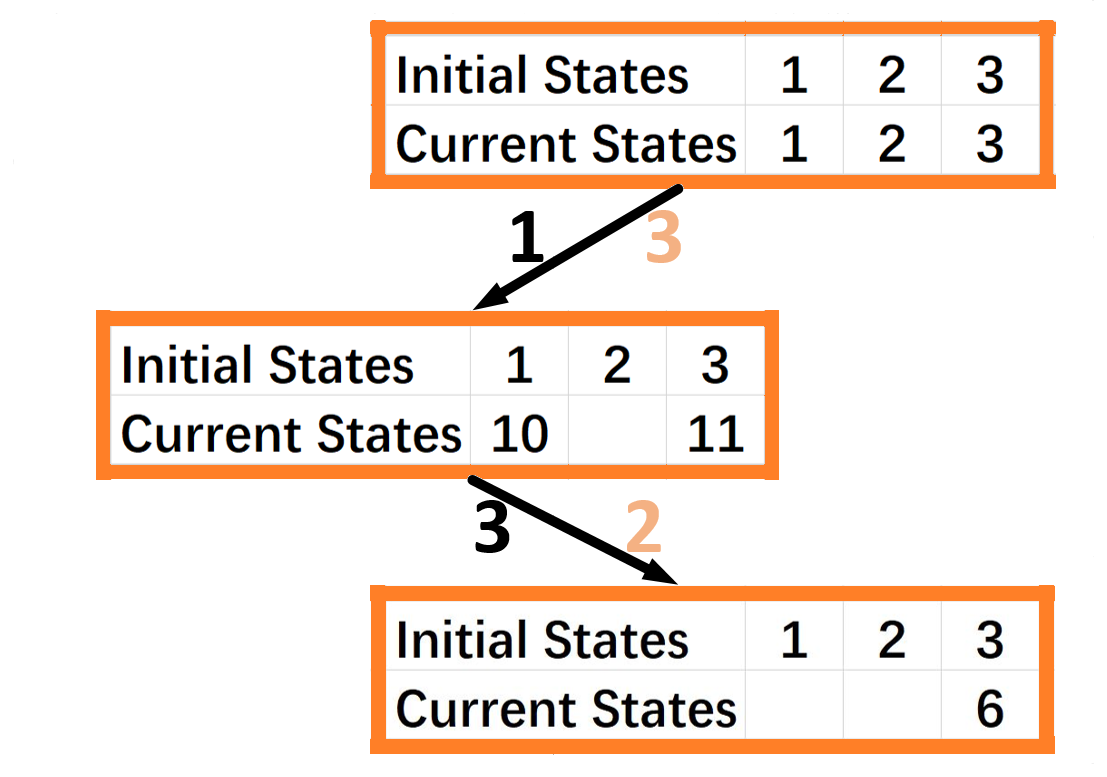
\includegraphics[scale=0.266]{figures/Fig5.png}}
	}}
      
      \caption{The process of determing the initial state of BCNs, we change the values of current states by input and the output we observe. }
      \label{fig:5}
   \end{figure}
%\subsection{Less observation costs}

Although the way of determine the initial state of a \BCN\ by the directed graph is very brief, but it would help us present how to do some optimization in the process of determining the initial state of the \BCNs.

